\documentclass[conference]{IEEEtran}

% Settings
\IEEEoverridecommandlockouts
\usepackage{cite}
\usepackage{amsmath,amssymb,amsfonts}
\usepackage{algorithmic}
\usepackage{graphicx}
\usepackage{textcomp}
\usepackage{xcolor}
\usepackage[hyphens,spaces,obeyspaces]{url}
\usepackage[colorlinks,allcolors=blue]{hyperref}

\graphicspath{ {../images/} }

\def\BibTeX{{\rm B\kern-.05em{\sc i\kern-.025em b}\kern-.08em
    T\kern-.1667em\lower.7ex\hbox{E}\kern-.125emX}}

\begin{document}

% Info

\title{Plant pathlology detection with convolutional neural networks\\ }

\author{
    \IEEEauthorblockN{Barış Deniz Sağlam}
    \IEEEauthorblockA{
        \textit{Informatics Institute} \\
        \textit{Middle East Technical University} \\
        Ankara, Turkey \\
        e155841@metu.edu.tr
    }
}

% Paper

\maketitle

\begin{abstract}
\end{abstract}

\begin{IEEEkeywords}
Deep Learning, CNN, Plant Pathology
\end{IEEEkeywords}

\section{Introduction}

Apple industry in U.S. has \$15 billion annual market size \cite{Thapa2020}. 
Various kinds of plant diseases cause significant economic losses. 
The manual diagnosis of apple plant diseases are laborous and expensive. 
Hence, computer vision-based methods have been developed to detect diseases from the images of leaves. 
The variations in imaging conditions such as backgrounds, lighting, and the large variety of visual symptoms are the main challenging aspects for these methods. 

In this paper, we investigate the performance of convolutional neural networks, 
specifically, we train ResNet \cite{ResNet2016} 
and EfficientNet \cite{EfficientNet} architectures with different scales, 
on detecting plant diseases from the images of apple leaves. 

\subsection{Dataset}
We use \href{https://www.kaggle.com/c/plant-pathology-2021-fgvc8/overview}{Plant Pathology 2021-FGVC8 dataset} \cite{Thapa2020} for training the models. 
The dataset consists of over $18,632$ RGB images, 
varying between $2592 \times 1728$ to $5184 \times 3456$ in size, 
and their labels. Each sample is labelled by experts with one or more disease types 
due to the fact that a plant may have multiple diseases. 

There are 4 kinds of plant disease existing in the dataset:
\begin{itemize}
\item \textit{Frog-eye leaf spot}
\item \textit{Powdery mildew}
\item \textit{Rust}
\item \textit{Scab}
\end{itemize}

Additionally, a sample is labelled as \textit{healthy} when no disease is spotted, 
and labelled as \textit{complex} when many diseases are spotted.

\begin{figure}
    \centerline{\includegraphics[width = 0.45 \textwidth]{samples-4x4.png}}
    \caption{Sample images and labels from the dataset}
    \label{fig:samples}
\end{figure}

As it can be seen from Fig.~\ref{fig:label-dist}., there is imbalance among labels in the dataset.

\begin{figure}
    \centerline{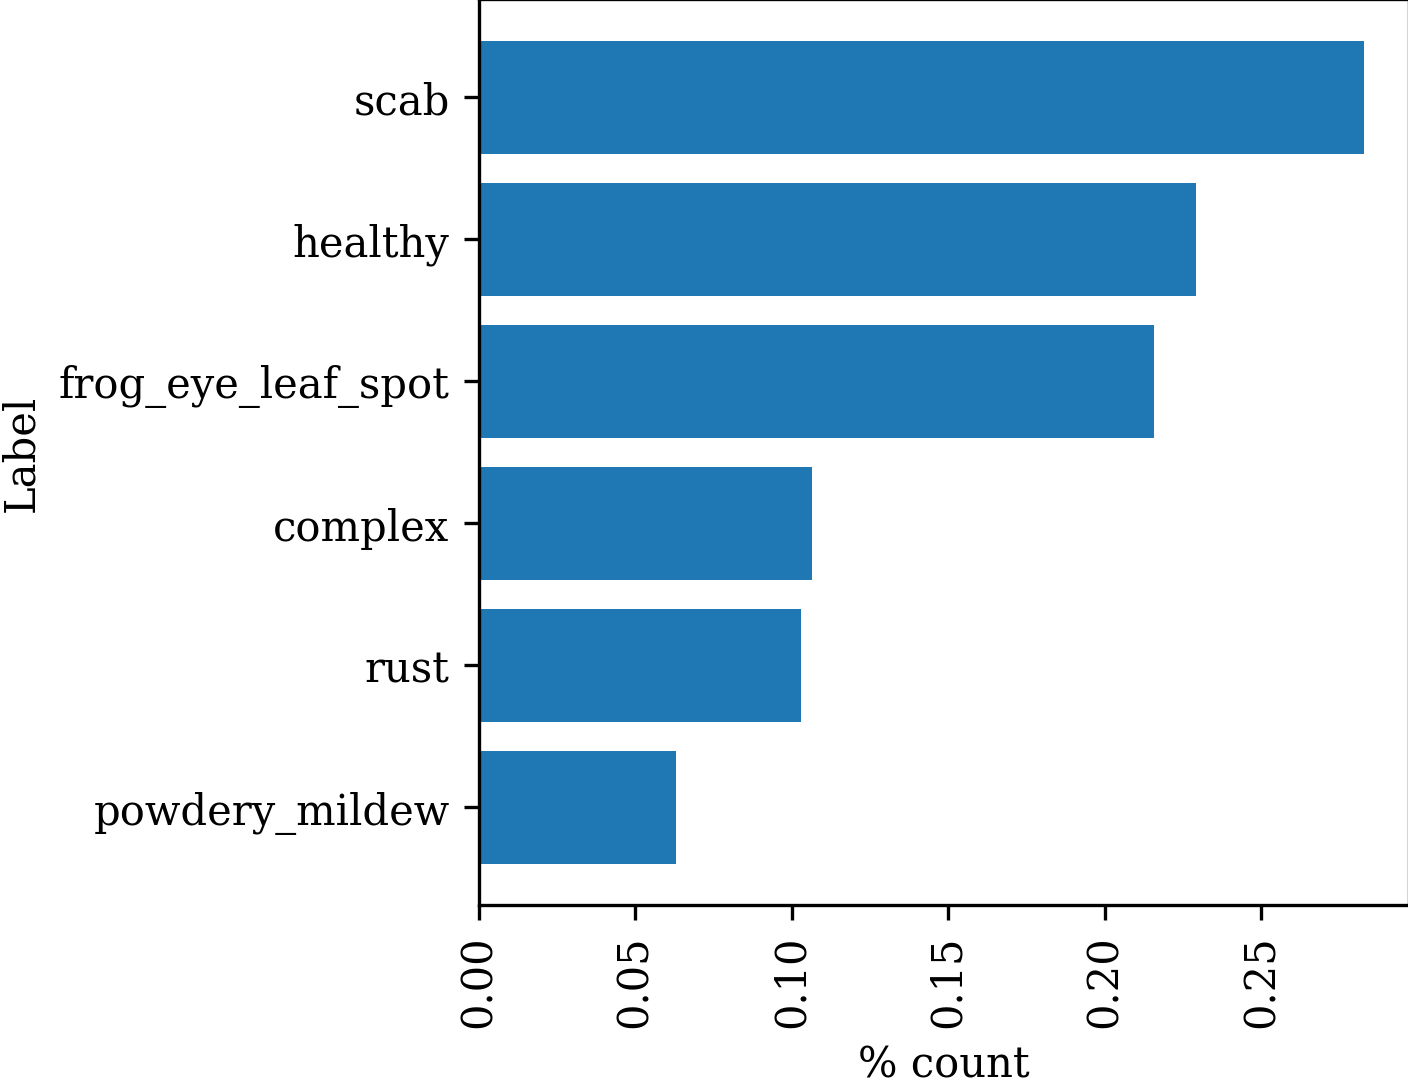
\includegraphics[width = 0.45 \textwidth]{label-dist-ratio.png}}
    \caption{Label distribution in the dataset}
    \label{fig:label-dist}
\end{figure}


\subsection{Literature Search}

Tan and Le \cite{EfficientNet} analyzed model scaling in convolutional neural networks 
and shown that when network depth, width, and resolution are balanced, the model performance
improves. They proposed a new scaling method parameterized with a single coefficient and
demonstrated that when the method is applied to scale existing CNNs such MobileNet, it 
achieves higher accuracy.
To test the effectiveness of the method on a novel model architecture, first, 
they perform a neural architecture search for a convolutional block constrained 
by number of FLOPs and create full networks by scaling this block with 
the proposed scaling method.
The family of such networks with different scales is named EfficientNets.
Then, they compare the performance of EfficientNets with other well-performing
convolutional neural networks such as 
ResNet \cite{ResNet2016}, 
InceptionNet \cite{InceptionNetV1} \cite{InceptionNetV3} \cite{InceptionNetV4}, 
and MobileNet \cite{MobileNet2017} 
on several image classification datasets such as 
CIFAR \cite{CIFAR}, and ImageNet \cite{ImageNet2014}. 
They show that EfficientNets achieve highest accuracy and faster inference on 
all datasets among all models with less parameters.

The paper by He et. al is a comprehensive ablation study on convolutional neural networks.
It investigates the impact of training techniques such as 
learning rate warming, label smoothing, transfer learning, weighting loss; 
and hyperparameters such as batch size, learning rate on three tasks image classification, 
object detection, and semantic segmentation with three CNN architectures
ResNet\-50 \cite{ResNet2016}, Inception\-V3 \cite{InceptionNetV3}, 
and MobileNet \cite{MobileNet2017}. The residual block of ResNet has convolutional layers 
with $1 \times 1$ kernel size and 2 stride, which ignores half of the information flowing throught the block \cite{BagOfTricks}. It also proposes a few modifications to 
Moreover, the convolutional layers with $7 \times 7$ kernel size are computationally 
more expensive than several successive $3 \times 3$ convolutions. Hence, the paper
proposes several tweaks to eliminate these inefficiencies in the original ResNet architecture.

Lin et al. \cite{FocalLoss} proposed a novel loss function that improves training accuracy in 
highly imbalanced problems such as object detection. Focal loss (Eq.\ref{eq:fl}) is a modulated 
cross entropy loss, where the modulating factor downweighs losses for easy 
negative examples such as background in object detection problems. This prevents 
easy negatives to dominate loss function and adversely influence the training.
The paper also proposes a one-stage object detection model architecture, named RetinaNet, 
that uses focal loss. It surpasses the accuracy of all two-stage object detection models 
without compromising inference speed and proves the effectiveness of focal loss.
We use focal loss in our models with the hyperparameters suggested by the paper.

\begin{equation*}
    p_T = 
    \begin{cases}
        p &\quad \text{if y = 1} \\
        1 - p &\quad \text{otherwise}
    \end{cases}
\end{equation*}

\begin{equation}
    \text{FL}(p_t) = \alpha_t (1 - p_t)^{\gamma}\log{p_t} \label{eq:fl}
\end{equation}

\section{Methods}

\subsection{Data quality}

\subsection{Model training and evaluation}
We trained several models with ResNet, EfficientNet and XResNet architectures 
with different model scales. Two model input sizes have been experimented; 
$384 \times 384 \times 3$ and $512 \times 512 \times 3$. 
The dataset is split into training and validation sets with 70-30\% ratios, respectively.
Since the task is multi-label classification, binary cross-entropy loss (Eq.\ref{eq:bce})
and focal loss (Eq.\ref{eq:fl}) functions have been used to train models. 
We trained a baseline model with ResNet18 architecture pretrained on ImageNet 
with no image augmentation and with binary cross entropy. 
\begin{equation*}
    \text{BCE} = -{(y\log(p) + (1 - y)\log(1 - p))} \label{eq:bce}
\end{equation*}

To improve model performance and training process, 
we utilized many techniques from \cite{BagOfTricks} and fastai \cite{fastai} library.
We used learning rate finder algorithm proposed by Smith \cite{Smith2015}
and implemented in fastai library to pick an optimal learning rate for fast convergence.
As learning rate scheduler, we used learning rate warmup and annealing \cite{BagOfTricks}
with 1cycle policy from \cite{Smith2018}. Alongside with focal loss, 
we experimented with weighted binary cross entropy loss with inverse 
frequencies of labels to mitigate the negative effects of class imbalance 
on model performance. 
Data augmentation is a common technique in deep learning practice due to its 
effectivess at preventing overfitting and improving model inference performance \cite{Shorten2019}.
We applied several image augmentation methods on our training set 
to increase generalization;
\begin{itemize}
    \item Horizontal and vertical flipping
    \item Translation
    \item 2D rotation
    \item Zoom in and zoom out
\end{itemize}

\begin{figure}[h]
    \centerline{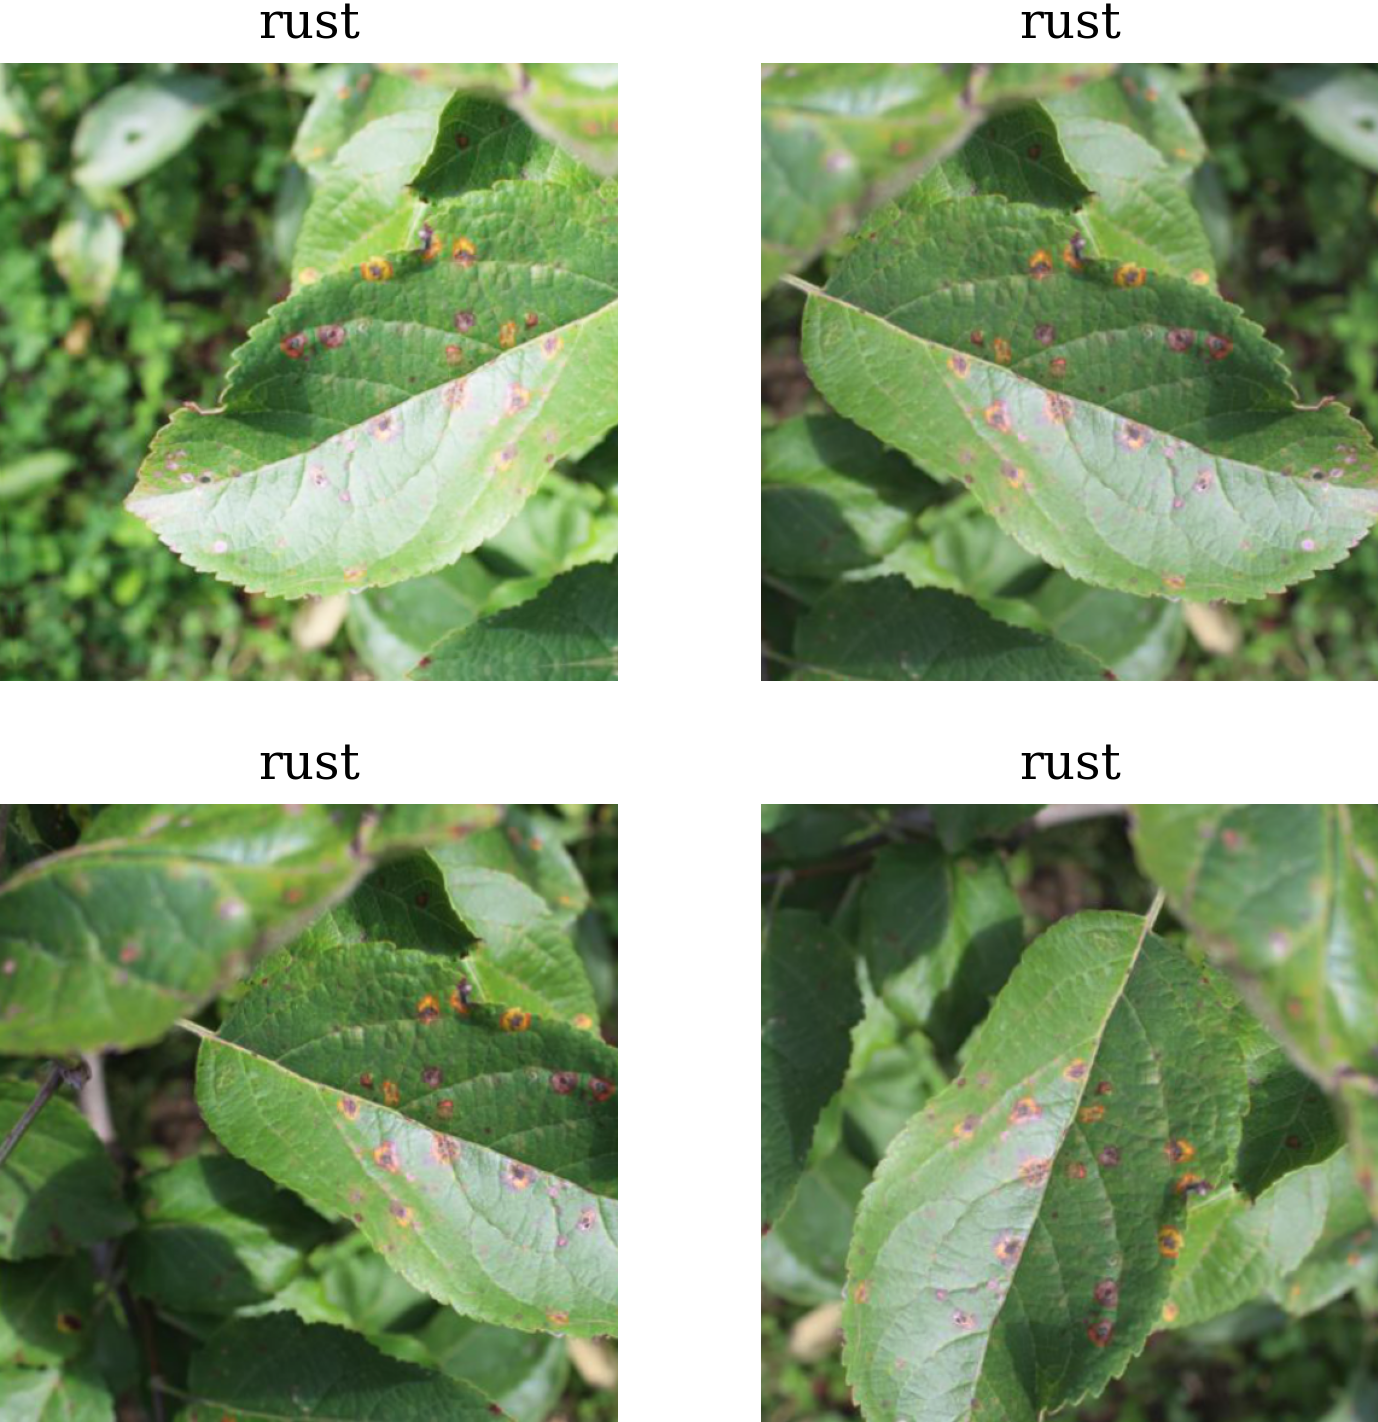
\includegraphics[width = 0.45 \textwidth]{image-aug-3x3.png}}
    \caption{Samples for the image augmentations applied on an image}
    \label{fig:image-aug}
\end{figure}

Low-precision floating point numbers (FP16) have been used 
for model weights and gradients to accelerate training 
\cite{Micikevicius2018} \cite{BagOfTricks}.
The models are evaluated with the following metrics implemented 
in scikit-learn library \cite{sklearn_api}: 
accuracy, F1 score with macro and samples averaging.

\begin{align*}
    \text{accuracy} &= \frac{TP+TN}{TP+TN+FP+FN} \\
    \text{F1} &= \frac{2*TP}{2*TP+FP+FN}
\end{align*}

\begin{table}[htbp]
\caption{Experiment results}
\begin{center}
\begin{tabular}{llll|rrr}
\textbf{Arch.} & \multicolumn{1}{l}{\textbf{Img size}} & \textbf{Aug.} & \textbf{Loss} & \multicolumn{1}{r}{\textbf{Acc.}} & \multicolumn{1}{r}{\textbf{F1(macro)}} & \multicolumn{1}{r}{\textbf{F1(samples)}} \\ \hline
ResNet18              & 384 & No                    & BCE     & 0.960                                 & 0.879                                  & 0.500                                       \\ 
ResNet34              & 384 & No                    & BCE     & 0.964                                 & 0.885                                  & 0.500                                       \\ 
ResNet18              & 384 & Light                 & BCE     & 0.959                                 & 0.871                                  & 0.500                                       \\ 
ResNet101             & 384 & Light                 & BCE     & 0.860                                 & 0.440                                  & 0.500                                       \\ 
EfficientNet-B0       & 384 & Light                 & BCE     & 0.954                                 & 0.862                                  & 0.647                                    \\ 
EfficientNet-B3       & 384 & Light                 & BCE     & 0.957                                 & 0.883                                  & 0.658                                    \\ \hline
\end{tabular}
\label{table:experiment_results}
\end{center}
\end{table}

\section{Conclusion}
\clearpage

\bibliographystyle{IEEEtran}
\bibliography{bibliography.bib}

\end{document}
